\documentclass[journal,twoside]{IEEEtran}


\usepackage{mfirstuc}
\usepackage{svg}
\usepackage{amsmath}
\usepackage{fixltx2e}
\usepackage{caption}
\usepackage{cite}
\usepackage{physics}
\usepackage{amsmath}
\usepackage{tikz}
\usepackage{mathdots}
\usepackage{yhmath}
\usepackage{cancel}
\usepackage{color}
\usepackage{xcolor}
\usepackage{siunitx}
\usepackage{array}
\usepackage{multirow}
\usepackage{amssymb}
\usepackage{gensymb}
\usepackage{tabularx}
\usepackage{extarrows}
\usepackage{booktabs}
\usetikzlibrary{fadings}
\usetikzlibrary{patterns}
\usetikzlibrary{shadows.blur}
\usetikzlibrary{shapes}





\begin{document}

\title{Design, Optimization and Implementation of a Not-So-Very-Simple Network Queueing Algorithm}


\author{Işık Emir~Altunkol, Özgür~Gülsuna,~\IEEEmembership{Undergraduate,~METU}}

% The paper headers
\markboth{\capitalisewords{Course of EE314, Middle East Technical University. 7 July~2022}}
{Design, Optimization and Implementation of a Not-So-Very-Simple Network Queuing Algorithm}
% The only time the second header will appear is for the odd numbered pages
% after the title page when using the twoside option.
% 
% *** Note that you probably will NOT want to include the author's ***
% *** name in the headers of peer review papers.                   ***
% You can use \ifCLASSOPTIONpeerreview for conditional compilation here if
% you desire.

\maketitle

% As a general rule, do not put math, special symbols or citations
% in the abstract or keywords.
\begin{abstract}
Network systems play a critical role in several operations in the information age. Immeasurable amount of data flow over the Internet makes it a difficult challenge for hardware to process the data in fast and reliable manner, often resulting in trade-offs between these requirements. Fortunately, a prioritization of these requirements can be decided for many types of data, and the network system can be optimized so that the requirements for each packet of data are satisfied as much as is feasible. This report focuses on the design, optimization and implementation of a queuing algorithm for a specific type of quality of service (QoS) network in which there are four buffers having different reliability and latency priorities. The proposed solution is to use a weighted decision algorithm in which each of the buffers have different reliability and latency parameters to model the requirement priority. To decide from which buffer to transmit data, a simple decision function is implemented using the weights and the state of the system at that moment. In order to test the viability of the algorithm, a simulation environment is created on MATLAB with the ability to test different input cases and system parameters. Furthermore, using the simulation outputs we implemented a cost function to minimize, and used the NSGA-II (Non-dominated Sorting Genetic Algorithm) algorithm to determine the optimized weights for the reliability and latency of the buffers. Finally, we implemented the design on an FPGA (Field-Programmable Gate Array) using Verilog HDL (Hardware Description Language) and observed the expected operation of the algorithm.
\end{abstract}

% Note that keywords are not normally used for peerreview papers.
\begin{IEEEkeywords}
queueing algorithm, networking, optimization, NSGA-II.
\end{IEEEkeywords}


\section{Introduction}
\IEEEPARstart{I}{n} communication networks, scheduling or queuing can be defined as a routine to arrange the data sequence in accordance with the criteria of the network. More briefly, the queuing algorithm decides on which packet to forward or which to drop; from this perspective, it plays a critical role in the streaming capabilities of the network. The network quality is described by the Quality of Service (QoS) measure. The QoS of the selected network may depend on various factors such as packet loss, packet error, packet latency, and packet delay variation. \\

\begin{figure}[ht]
    \centering
    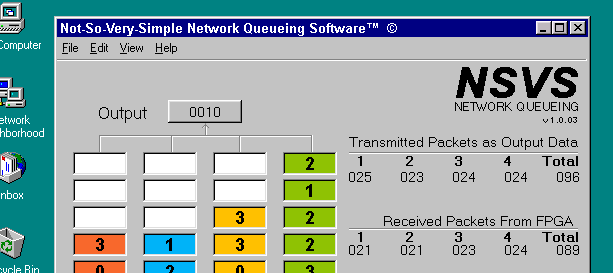
\includegraphics[width=0.95\linewidth]{figures/fig_vga_4.png}
    \captionsetup{justification=centering}
    \caption{User Interface for the Overall System Implemented on FPGA}
    \label{fig:VGA}
\end{figure}


\indent Our problem definition selects packet latency and packet loss/drop as the only factors over a buffering structure consisting of four parallel linear buffers, each with six packets, working in a first-in-first-out manner. The buffer network is visualized in Fig. \ref{fig:buffer}. The exemplary network requires three specifications, Latency precedence, Reliability precedence, and minimum packet loss. Latency precedence can be explained as the most up-to-date packets over the buffers should be arranged as the condition in \ref{Latency}.
\begin{equation}\label{Latency}
L_{1} < L_{2} < L_{3} < L_{4}
\end{equation}

\indent Similarly, reliability precedence is that the least amount of drops should occur in buffer four with decreasing order as in \ref{Reliability}.
\begin{equation}\label{Reliability}
R_{4}  >R_{3}  >R_{2}  >R_{1}
\end{equation}

\indent The final specification is that overall drops should be minimized for all buffers. Another property of the exemplary system is data output rate, which is fixed at 3 seconds. There exist numerous algorithms with generalized performance over the implemented medium. The test environment for our algorithm to run is selected as FPGA, which is a configurable integrated circuitry dedicated to implementing logic circuit elements.\\

\indent In this paper, a weighted selection algorithm is designed, optimized for randomized inputs with average congestion on the network using the NSGA-II algorithm, and finally implemented on Altera DE1-SoC FPGA with a visual user interface over the VGA (Video Graphics Array) shown in Fig. \ref{fig:VGA}. Section II discusses the design of the queuing algorithm, Section III discusses the determination of weights using optimization, and Section IV discusses the implementation of the algorithm on FPGA environment. Finally, the conclusions are drawn in Section V.

\begin{figure}[ht]
    \centering
    \includesvg[width=0.9\linewidth]{figures/buffer.svg}
    \captionsetup{justification=centering}
    \caption{Exemplary Buffer Structure}
    \label{fig:buffer}
\end{figure}


\section{Design of the Queuing Algorithm}
\subsection{The Algorithm}
\indent Implementing an algorithm according to such requirements is surprisingly tricky due to the conflicting latency and reliability requirements and the system's strong performance dependence on the ingress data traffic. Considering the case where the data input rate is higher than the output rate, the buffers would swell after some time. The cost of holding the requirements will be in jeopardy at that condition. Similarly, in the case of slow data input, the buffers will be almost empty, and the requirements will also become meaningless. Due to these difficulties, the data input for our system is selected as randomized inputs at a changing rate with an average input rate equal to the average output rate.\\

\indent In the essence of the decision algorithm, there lies a need to select in which buffer to read from every three seconds. Our approach is to find a decision function that can be calculated for each buffer individually, utilizing adjustable weights. The buffer with the highest decision function value is then selected. Two state variables are defined to be used in the decision function. The first one is present buffer fullness denoted by $f$. The second one is the latency decision variable denoted by $t$, which can be described as the summation of the times spent since the packet arrival for each packet at that buffer.\\

\indent For two criteria, latency and reliability, we also have two weights. The latency weight is multiplied by the latency decision variable for the corresponding buffer. The reliability weight is multiplied by the square of the fullness of that buffer. Reliability and latency components are summed to result in the decision function $D$, which is visualized in matrix function notation in \ref{DecisionFunciton}.\\
\begin{equation}
\begin{array}{l}
\begin{bmatrix}
D_{1}\\
D_{2}\\
D_{3}\\
D_{4}
\end{bmatrix} =\begin{bmatrix}
\ \ \ \ W_{L1} \cdotp t_{1} \ \  & + & \ \ \ \ W_{R1} \cdotp f{_{1}}^{2} \ \ \ \ \\
\ W_{L2} \cdotp t_{2} & + & \ \ W_{R2} \cdotp f{_{2}}^{2} \ \ \\
W_{L3} \cdotp t_{3} & + & \ \ W_{R3} \cdotp f{_{3}}^{2} \ \ \\
W_{L4} \cdotp t_{4} & + & \ \ W_{R4} \cdotp f{_{4}}^{2} \ \ 
\end{bmatrix}
\end{array}
\label{DecisionFunciton}
\end{equation}\\
The  latency decision variable takes the overall amount of latency into account in the decision function. The fullness is squared to model the increasing risk of a packet drop as the buffer fullness increases.

\subsection{Numerical Simulation}
\indent Before implementing the algorithm in the physical system, it is tested in a simulation environment where performance is evaluated similarly to the requirements. The precedences of latency and reliability are one criterion, and overall drop count is another. One important notice is that in performance grading, drop per input is used instead of total drop count, and average latency over the input is used instead of total latency count. Taking the average of performance variables eliminates the performance variables' dependence on the number of inputs. The simulation environment is tested with inputs consistent with the considerations mentioned earlier. The simulation process showed that the requirements could be met with appropriate weights.


\section{Optimization: Determination of Weights}

The system performance is strongly determined by the latency and reliability weights. As these weights can be of any value, one should find an optimum set of weights for the algorithm to work in the desired way. The parametric sweep is not an option due to the high number of parameters and multiple objectives to achieve. Hence, one could use a multi-objective optimization algorithm to optimize the operation. We decided to use the NSGA-II optimization algorithm, which is a fast and elitist multi-objective genetic algorithm \cite{NSGA}.\\

\indent The first step of a multi-objective optimization is the determination of the cost functions (i.e. objective functions). System is aimed to be optimized according to three objectives: The latency and reliability criteria given in \ref{Latency} and \ref{Latency}, together with having a minimal amount of packet drops. Since there is a simulation environment, one can use it to implement the cost functions using the simulation outputs. The latency and reliability weights of the buffers are chosen as the optimization parameters, hence there should be 8 parameters. These parameters are inputted to the objective function which is able to run a simulation using these parameters. After every simulation, the drop per input (DPI) and average latency values for every buffer are calculated. To obtain the normalized average latency (NAL) values, all of the average latency values are divided to the value of the maximum one. Network administrators may model the cost function in various ways for different networks. According to the criterion \ref{Reliability} and \ref{Latency}, different cost functions are considered, and finally it is decided to model the cost for drop and latency as in equations \ref{cost_fn_reliability} and \ref{cost_fn_latency} respectively.

\begin{equation} \label{cost_fn_reliability}
C_{reliability} =  \sum_{i=1}^{4} 1000e^{50(DPI_{i+1}-DPI_{i})}
\end{equation}

\begin{equation} \label{cost_fn_latency}
C_{latency} =  \sum_{i=1}^{4} 1000e^{50(NAL_{i}-NAL_{i+1})}
\end{equation}

\begin{table*}[ht]
\begin{tabular}{cccc|cccc||ccc}
\toprule 
$\displaystyle W_{L1}$ & $\displaystyle W_{L2}$ & $\displaystyle W_{L3}$ & $\displaystyle W_{L4}$ & $\displaystyle W_{R1}$ & $\displaystyle W_{R2}$ & $\displaystyle W_{R3}$ & $\displaystyle W_{R4}$ &  Latency Objective  &  Reliability Objective  & $\sum$ DPI \\
\midrule 
 0.0715 & 0.06 & 0.035 & 0.0169 & 0.0000 & 0.2165 & 0.5635 & 0.9354 & 25.8719 & 15.949 & 0.9756 \\
\colorbox{yellow}{0.0758} & \colorbox{yellow}{0.0626} & \colorbox{yellow}{0.0385} & \colorbox{yellow}{0.0116} & \colorbox{yellow}{0.0000} & \colorbox{yellow}{0.2011} & \colorbox{yellow}{0.5735} & \colorbox{yellow}{0.9704} & \colorbox{yellow}{10.9687} & \colorbox{yellow}{25.5297} & \colorbox{yellow}{0.9729}\\
0.0813 & 0.0545 & 0.0274 & 0.0000 & 0.0000 & 0.3165 & 0.5539 & 0.9269 & 6.6714 & 86.7803 & 0.9706 \\
0.0881 & 0.0687 & 0.0280 & 0.0045 & 0.0000 & 0.2338 & 0.7031 & 1.0000 & 4.1226 & 35.2729 & 0.9652 \\
0.0720 & 0.0526 & 0.0228 & 0.0000 & 0.0041 & 0.3797 & 0.7513 & 0.9882 & 3.1962 & 90.888 & 0.9632 \\
 \bottomrule
\end{tabular}
\caption{Optimized Weights in Tabular Form with Selected Weight Set Underlined}
\label{opt_weigths}
\end{table*}

To understand the cost function, one may inspect the $1000e^{50(DPI_{i+1}-DPI_{i})}$ expression from equation \ref{cost_fn_reliability}. For instance, as the drop per input for the fourth buffer increases and approaches the value of the third one, the difference $DPI_{4}-DPI_{3}$ starts to approach 0 and even if $DPI_{4}$ gets slightly larger than $DPI_{3}$ the exponential expression increases rapidly, causing a dramatic increase in cost.
The numbers 1000 and 50 are chosen to shift the point on which the exponential function is equal to 1 and tune the rate of increase of the function to a desired amount. A similar calculation is done for every buffer and summed up to calculate $C_{reliability}$. The same procedure is applied to determine $C_{latency}$ in \ref{cost_fn_latency}. Furthermore, the exponential function gives a smooth and positive definite cost function which makes it easier for the optimization algorithm to minimize. Finally, equation \ref{cost_fn_drop} is used to model the overall cost for the drop counts.




\begin{equation} \label{cost_fn_drop}
C_{drop} = \sum_{i=1}^{4} DPI_{i}
\end{equation}

One of the challenges of the optimization is that eight parameters bring an enormous amount of computational burden. Hence, constraints should be determined for the optimization to run efficiently. The constraints are deduced from the assumptions \ref{reliability_assumption} and \ref{latency_assumption}, that is, the for the requirements to be satisfied as in conditions \ref{Reliability} and \ref{Latency} the weights are assumed to follow a similar pattern.

\begin{equation} \label{reliability_assumption}
W_{R4}  >W_{R3}  >W_{R2}  >W_{R1}
\end{equation}

\begin{equation} \label{latency_assumption}
W_{L4}  <W_{L3}  <W_{L2}  <W_{L1}
\end{equation}

To further reduce the computational burden, it is necessary to specify the range in which the optimization parameters are searched. Considering the constraints and the structure of the decision function we guessed and tried out some feasible parameter values on the simulation environment. According to the results, we determined a viable range to search the parameters.\\

\indent For the optimization procedure, generation size is selected as 150 with population size of 100. Corresponding simulation parameters are, 20000 seconds of simulation for 6600 equal probabilistic random distributed inputs. Numerous of optimized weights are exhibited in Table \ref{opt_weigths} with selected weight set highlighted. Pareto surface corresponding to the optimization is presented in Fig. \ref{fig:pareto} with the polynomial surface is fitted on with a root mean square error (RMSE) of 0.008214. The fit also shows that the reliability and latency requirements are more greatly met with not unnoticeable change on the overall drop per input. The highlighted set is selected as design weights to be implemented.


\begin{figure}[ht]
    \centering
    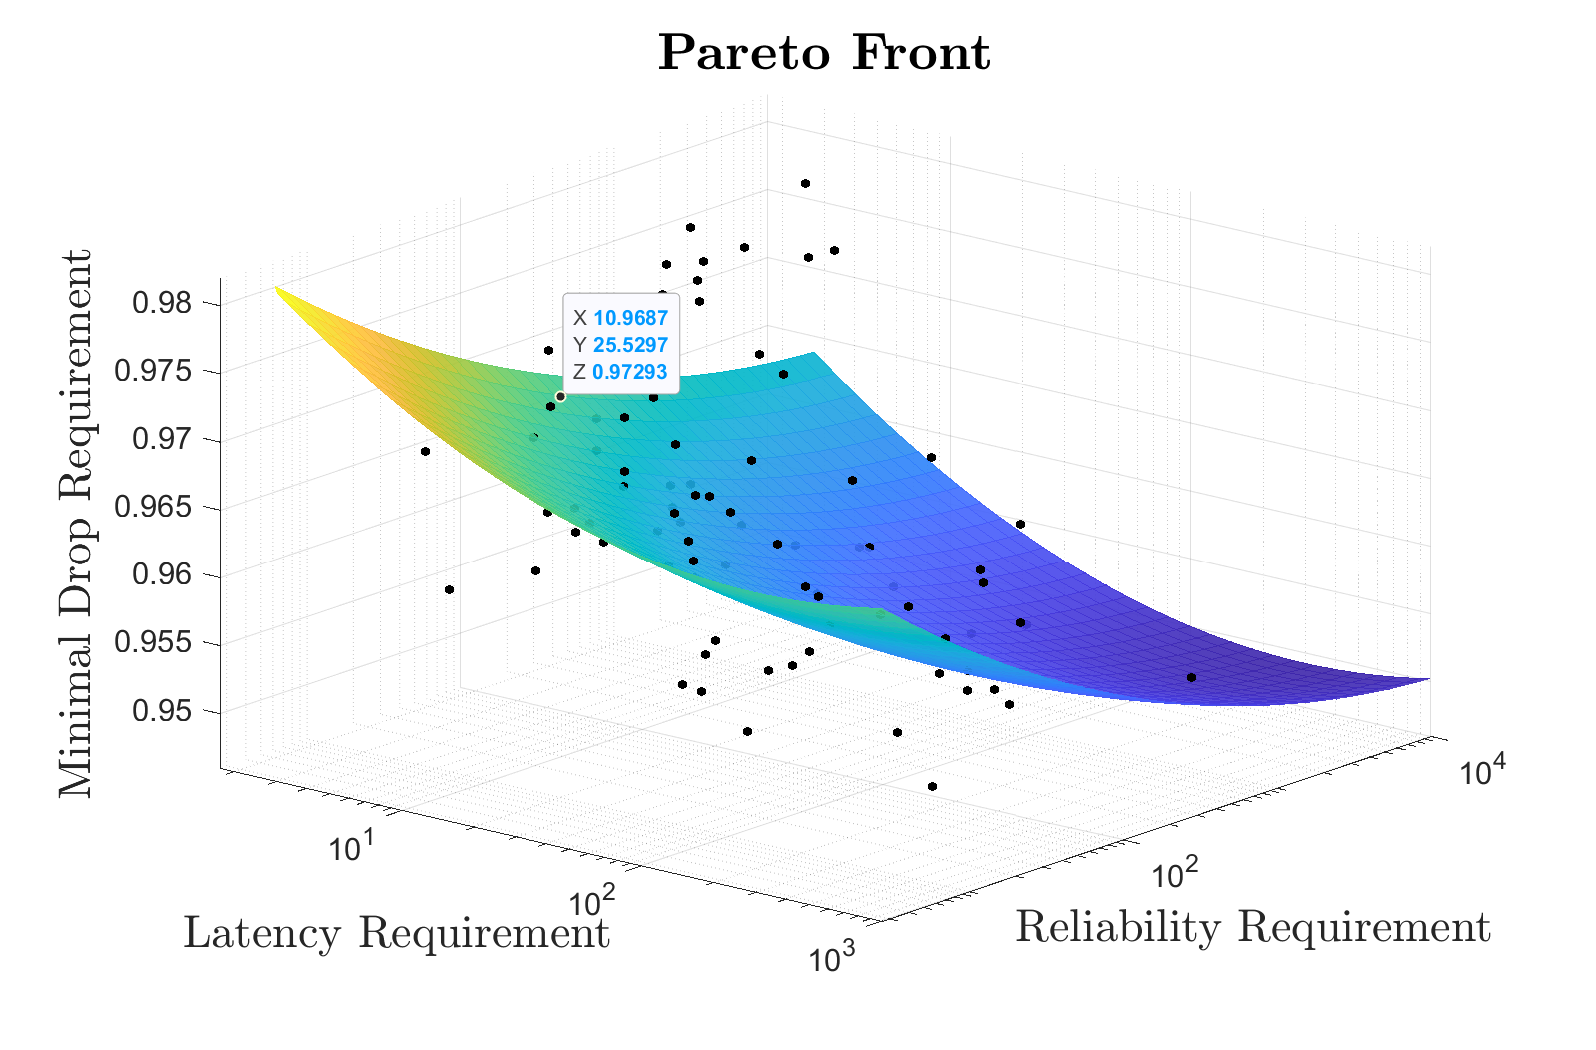
\includegraphics[width=1.1\linewidth]{figures/pareto.eps}
    \captionsetup{justification=centering}
    \caption{Pareto Frontier of the optimization with selected set highlighted}
    \label{fig:pareto}

\end{figure}




\indent The algorithm with the optimized weight set is then simulated in the same simulation environment to verify the requirements. Output of the simulation can be seen in Table \ref{ALDPI} which clearly shows that the selected weights are applicable.

\begin{table}
    \centering
    \scalebox{1.2}{ %This is for scaling.
        \begin{tabular}{|c|c|c|c|}
        \hline 
         \multicolumn{4}{|c|}{Average Latency (AL)} \\
        \hline 
         102.39 & 106.36 & 124.95 & 145.05 \\
        \hline\hline 
         \multicolumn{4}{|c|}{Drop Per Input (DPI)} \\
        \hline 
         0.3526 & 0.3324 & 0.2070 & 0.1036 \\
         \hline
        \end{tabular}
        }
\caption{Simulation Result with The Optimized Weights}
\label{ALDPI}
\end{table}

\vspace{-0.2em}
    
\section{Implementation on FPGA}

A modular approach is used to implement the algorithm in a way that is easier to test and debug. The main Verilog module is composed of six different Verilog modules: buffer module, switch module, decision module, clock divider module, debouncer module, and VGA module. The operation of each module will be explained and necessary simulation results will be demonstrated in this section.\\

\indent The overall system will operate in sequential logic. The $50MHz$ internal clock signal of the FPGA is used to synchronize the circuit. However, lower frequency clock signals are required for several operations. Hence, a simple clock divider module is implemented. It takes the $50MHz$ clock signal as input. The outputs are a $25MHz$ clock for the VGA operation, a $20Hz$ "fractional clock" for the debouncer, and a "read clock" with a period of 3 seconds.\\

\indent The buffer module implements the buffers. A fractional clock, a 4-bit parallel data input, a read signal, and a write signal is inputted to this module. The buffer module has a 24-bit output register to model the ability to store six packets of 4-bit data. Also, the buffer fullness, the latency decision parameter, the input count, and the drop count are calculated inside this module and outputted. The buffer is implemented as follows: Every time the write input is 1 before the rising edge of the fractional clock, parallel input is written to the next empty slot of the buffer. If the buffer is full, the oldest data is dropped by shifting the packets through the slots, and the new one is written to the last slow. Also, when a read signal occurs, the packets are shifted in the same way so that the oldest data is dropped after the read operation. Hence, the buffer works in a first-in first-out manner. The calculation of the fullness and the drop count are straightforward. We defined "time counter" registers for every packet slot to count the rising edges of the clock ever since a packet arrived. Finally, they are summed up to evaluate the latency decision parameter. The simulation for the buffer module is given in Fig. \ref{fig:buffer_decision_simulation}, simulated together with the decision module.\\

\indent The switch module processes the input data from the FPGA buttons so that the serial input is converted to a 4-bit parallel input, and sent to the appropriate buffer. The module has a fractional clock input, a start input, a serial 0 input and a serial 1 input. It outputs the write signals and the parallel data input for the buffers. The module detects when the start button is pressed using the rising edges of the start signal. These rising edges imply that the system will wait until it receives four inputs from the serial 0 and serial 1 buttons. The inputs are also received using rising edge detection, from the LSB (Least Significant Bit) to MSB (Most Significant Bit). After the four inputs are received, they are outputted to the 4-bit parallel output register, and the write signals are configured. To determine the write signals, the two MSBs of the input data is checked. Operation of this unit, together with the debouncer module, is validated with the simulation result in Fig. \ref{fig:switch_simulation}.

\begin{figure}[ht]
    \centering
    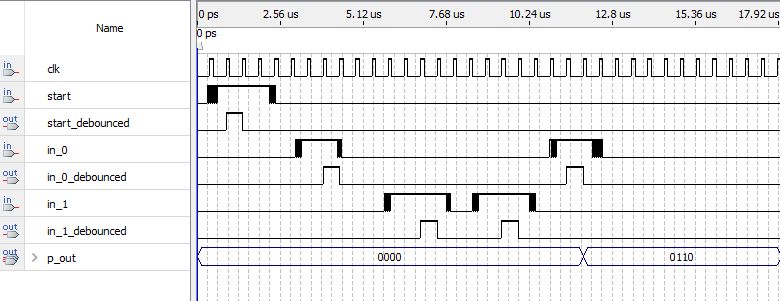
\includegraphics[width=0.95\linewidth]{figures/button_test.png}
    \captionsetup{justification=centering}
    \caption{Simulation Waveform of the Switch and Debouncer Modules}
    \label{fig:switch_simulation}
\end{figure}

The buttons on FPGA will cause bouncing in the input signals. To avoid this circumstance, the debouncer module takes an input signal and creates an output pulse with a single clock period width for every rising edge of the input. Additionally, the bouncer should have a clock input which has a long enough period to avoid the bouncing signal. Hence, the fractional clock is inputted to this module. This debouncer implementation is both simulated and tested on the FPGA together with the switch module.\\

\indent The decision module implements the decision function by taking the necessary inputs (buffer fullnesses, latency decision parameters, read clock and fractional clock signals), and outputs the read signals for the buffers. Optimized weights are hard-coded in the module. To avoid floating point operations while preserving the precision, weights are multiplied with 1000 before the implementation. This module is simulated together with the buffer module, and the results are in Fig. \ref{fig:buffer_decision_simulation}.

\begin{figure}[ht]
    \centering
    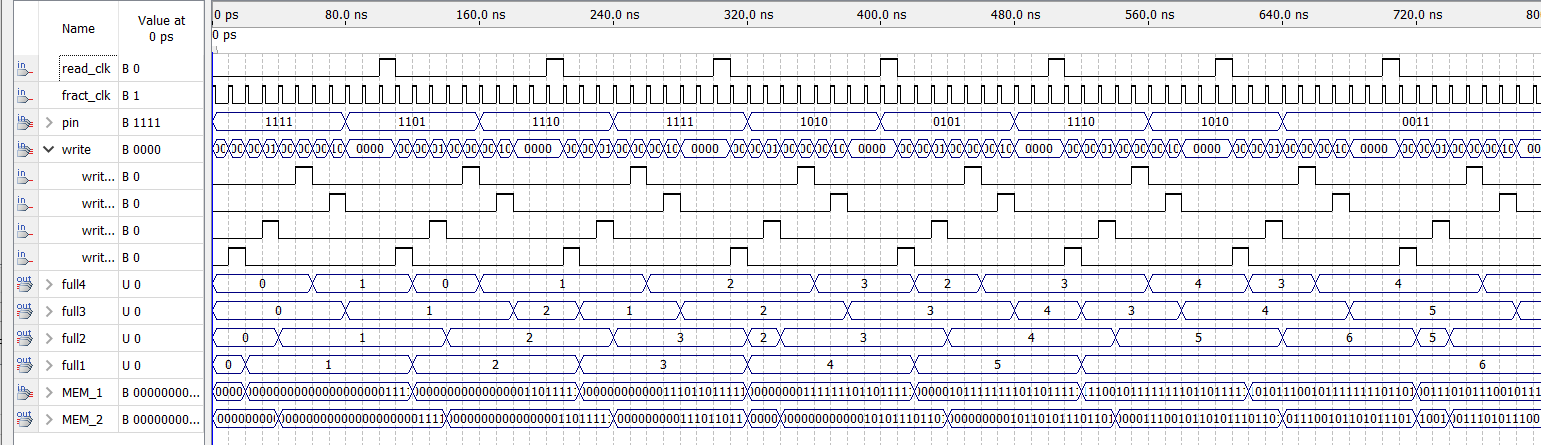
\includegraphics[width=0.95\linewidth]{figures/buffer_decision_sim.PNG}
    \captionsetup{justification=centering}
    \caption{Simulation Waveform of the Buffer and Decision Modules}
    \label{fig:buffer_decision_simulation}
\end{figure}

The VGA module is responsible for running the interface of the algorithm. It has many inputs, since it uses most of the variables to print them on the screen. After making necessary calculations, it gives five critical outputs: three 8-bit signals for red, green, and blue; vertical synch and horizontal synch signals. Since the 640 x 480 pixels $60Hz$ VGA standard is used, the horizontal and vertical synch signals are configured as specified in the standard. RGB (Red Green Blue) signals are determined using the state of the system and the design of the interface. Our interface had a background image, which included a Windows 95 screen, the empty buffers and the constant texts. Also, as input data are written to the buffers, the buffers are filled with the data with a different background color for every buffer. At the right part of the screen, the number of transmitted packets, received packets and drop counts are written.\\

\vspace{1em}

\begin{figure}[b]
    \centering
    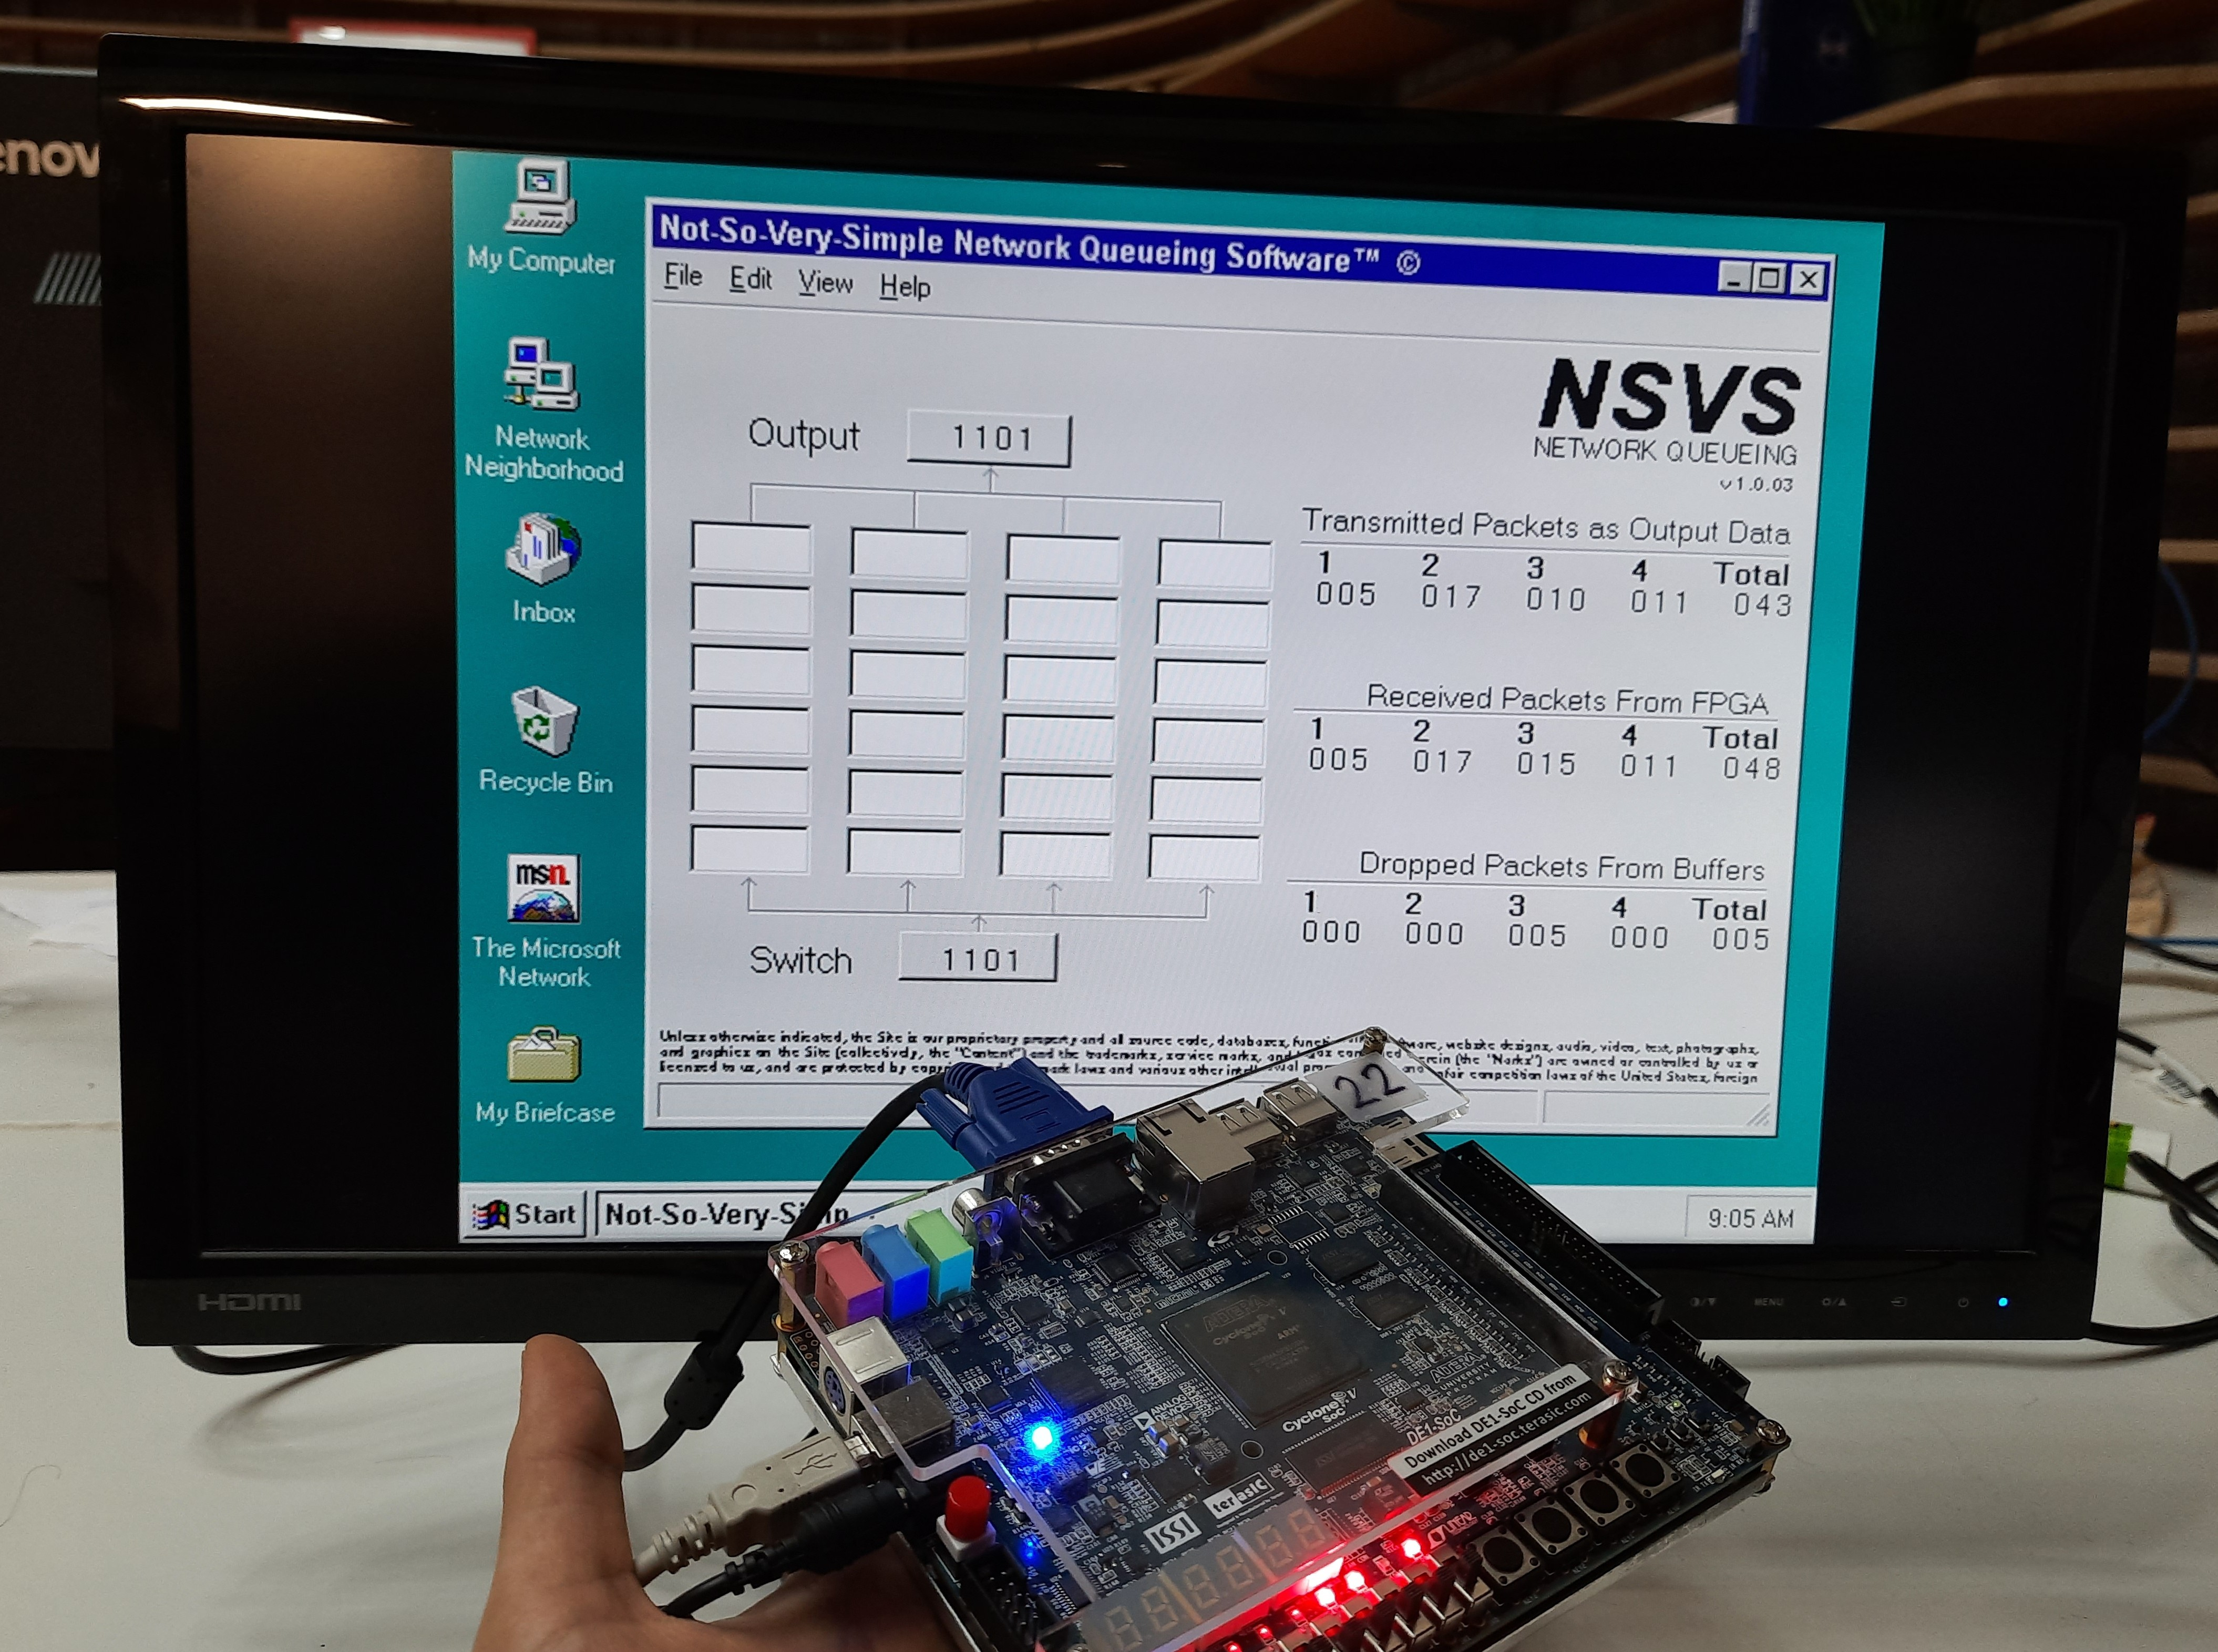
\includegraphics[width=0.95\linewidth]{figures/FFFPPPGGGA.jpg}
    \captionsetup{justification=centering}
    \caption{System as a Whole}
    \label{fig:fpga}
\end{figure} 

\indent After implementing and testing the modules separately, we connected them in the main module, compiled it, and tested it on the FPGA. The algorithm worked as expected.\\

\indent One of the problems with implementing VGA module is that there are lots of pixels and lots of bits for every pixel. We coded a bitmap to .mem file converter (and .mem file to bitmap converter) using Python. We converted our background image to a bitmap and then converted it to a .mem file, and observed that it has 307.200 lines of 8-bit data for every color. This amount of data increases the compile time enormously which would make it impossible to test and debug the module. To help us with the situation, we modified the .mem converter script to be able to compress the images to 1-bit from 8-bit, by only considering their most significant bits. Also, using the converter as a simulation tool, we observed that a 3-bit image is more than enough for our choice of colors. Hence, we compressed the images to 3-bits on our final implementation.\\




\section{Conclusion}
This paper discusses the design, optimization, and implementation of a queueing algorithm. The problem is defined around the requirements and limitations. An exemplary decision function is constructed and tested in a simulation environment. Later weights are optimized using a genetic algorithm, more precisely NSGA-II, in a multi-objective manner. It is shown that the decision function is capable of satisfying the requirements. Moreover, with the optimized weights of the decision function, it is ensured that the algorithm's performance is at its top level. At last, the queuing algorithm is implemented on FPGA with inputs from buttons and output to the user using the VGA interface. The system as a whole can be seen in the Fig. \ref{fig:fpga}. \\ 

\indent Further development of this algorithm includes input data model identification and adaptive modification of the weights with changing network characterization.


\bibliographystyle{IEEEtran}
\bibliography{refs.bib}



\end{document}


